\documentclass[review]{elsarticle}


%% The amssymb package provides various useful mathematical symbols
\usepackage{amssymb}
\usepackage{natbib}
\usepackage{graphicx}
\usepackage{amsmath}
\usepackage{tabularx}
\usepackage{gensymb}
\usepackage[utopia]{mathdesign}
\usepackage[OMLmathrm,OMLmathbf,OMLmathsf,sfdefault=fav,scaled=0.875]{isomath}
\usepackage{color} % needed for the color change in TODO
\usepackage{gensymb} % needed for the degree C
%\usepackage{mathtools} 
\usepackage{caption}
\usepackage{subcaption}
\usepackage{epstopdf}
\usepackage{nomencl}
% \usepackage{german}
\usepackage{verbatim} 
\usepackage{xpatch}
\usepackage{framed} % Framing content
\usepackage{multicol} % Multiple columns environment
\makenomenclature%makeindex [].nlo -s nomencl.ist -o [].nls
\setlength{\nomlabelwidth}{.2\hsize}

\renewcommand{\nompreamble}{Throughout the article bold face symbols denote tensors and vectors. Normal face letters represent scalar quantities.}

\setlength{\nomitemsep}{-\parsep}

%Define groups for nomenclature

\RequirePackage{ifthen}

\renewcommand{\nomgroup}[1]{\bigskip%

\ifthenelse{\equal{#1}{R}}{\item[\textit{Roman symbols}]}{%

\ifthenelse{\equal{#1}{G}}{\item[\textit{Greek symbols}]}{\ifthenelse{\equal{#1}{O}}{\item[\textit{Operators}]}}}}


\newcommand{\tm}{\textrm}
\newcommand{\var}{\varepsilon}
\newcommand{\si}{\sigma}
\newcommand{\beq}{\begin{equation}}
\newcommand{\eeq}{\end{equation}}
\newcommand{\nn}{\nonumber}
\newcommand{\mwith}{\quad \mathrm{with} \quad}
\newcommand{\mand}{\quad \mathrm{and} \quad}
\newcommand{\mdiv}{\,\mathrm{div}\,}
\newcommand{\mDiv}{\,\mathrm{Div}\,}
\newcommand{\grad}{\,\mathrm{grad}\,}
\newcommand{\Grad}{\,\mathrm{Grad}\,}
\newcommand{\Cel}{\,$^\circ$C}
\newcommand{\dcdot}{\mbf{\,:\,}}
\newcommand{\tr}{\mathrm{tr}\,}
\newcommand{\mathd}{\mathrm{d}}
\newcommand{\mathD}{\mathrm{D}}
\newcommand{\mdiag}{\,\mathrm{diag\,}}
%\newcommand{\mbf}[1]{\mbox{${\mbox{\boldmath${#1}$\unboldmath}}$}}
\newcommand{\fourtens}[1]{\mbox{${\mbox{\boldmath$\mathcal{#1}$\unboldmath}}$}}
\newcommand{\mbf}[1]{{\mathbf{#1}}}%tensors/matrices
\newcommand{\mbfs}{\boldsymbol}
\newcommand{\dev}{\stackrel{def}{=}}
\newcommand{\tbf}{\textbf}
\newcommand{\tit}{\textit}
\newcommand{\mrm}{\mathrm}
%\newcommand{\citep}[1]{(\cite{#1})}
%\newcommand{\citet}{\cite}

\newcommand{\tf}{$\rightarrow\ $}
\newcommand{\ds}{\displaystyle}
\newcommand{\mtd}[2]{\frac{\mathd_{#1}{#2}}{\mathd t}} %material time derivative
\newcommand{\ptd}[1]{\frac{\partial {#1}}{\partial t}} %partial time derivative
\newcommand{\pd}[2]{\frac{\partial {#1}}{\partial {#2}}} %partial derivative
\newcommand{\vint}[1]{\int \limits_\Omega {#1} \mathd \Omega} %volume integral
\newcommand{\sint}[2]{\int \limits_{\partial \Omega_{#1}} {#2} \mathd \Gamma}
\newcommand{\uexp}[1]{$^{\mathrm{{#1}}}$}%superscript
\newcommand{\uind}[1]{$_{\mathrm{{#1}}}$}%subscript

%\newcommand{\mvec}[1]{\uline{{#1}}}%Vektoren
%\newcommand{\mmat}[1]{\uuline{{#1}}}%Matrizen

\newcommand{\mvec}[1]{\mathsfbfit{#1}}%Vektoren
\newcommand{\mmat}[1]{\mathsfbfit{#1}}%Matrizen


\newcommand{\drop}[1]{\red \cancelto{0}{\black #1} \black}

\newcommand{\centerpic}[3]{\hspace{#1\textwidth}\resizebox{#2\textwidth}{!}{\includegraphics{#3}}}

\newcommand{\squote}[2]{\begin{quote}{\huge{``}}{#1}{\huge{''}}\end{quote}\hfill Aus: {#2}}

\newcommand{\todo}[1]{\textcolor{red}{#1}}
\newcommand{\correction}[1]{\textcolor{blue}{#1}}

\newcommand{\comments}[1]{\textcolor{blue}{#1}}

\usepackage{lineno,hyperref}
\modulolinenumbers[5]

\journal{Water Resource Research}

%%%%%%%%%%%%%%%%%%%%%%%
%% Elsevier bibliography styles
%%%%%%%%%%%%%%%%%%%%%%%
%% To change the style, put a % in front of the second line of the current style and
%% remove the % from the second line of the style you would like to use.
%%%%%%%%%%%%%%%%%%%%%%%

%% Numbered
%\bibliographystyle{model1-num-names}

%% Numbered without titles
%\bibliographystyle{model1a-num-names}

%% Harvard
%\bibliographystyle{model2-names.bst}\biboptions{authoryear}

%% Vancouver numbered
%\usepackage{numcompress}\bibliographystyle{model3-num-names}

%% Vancouver name/year
%\usepackage{numcompress}\bibliographystyle{model4-names}\biboptions{authoryear}

%% APA style
%\bibliographystyle{model5-names}\biboptions{authoryear}

%% AMA style
%\usepackage{numcompress}\bibliographystyle{model6-num-names}

%% `Elsevier LaTeX' style
\bibliographystyle{elsarticle-num}
%%%%%%%%%%%%%%%%%%%%%%%

\begin{document}

\begin{frontmatter}

\title{Analytical analysis of timescales of seawater intrusion and retreat}
%\tnotetext[mytitlenote]{Fully documented templates are available in the elsarticle package on \href{http://www.ctan.org/tex-archive/macros/latex/contrib/elsarticle}{CTAN}.}

%% Group authors per affiliation:
\author[label1,label2]{Tianyuan Zheng}
\ead{tianyuan.zheng@ufz.de}
\author[label3]{Bo Guo\corref{cor1}}
\ead{boguo@princeton.edu}
\cortext[cor1]{Corresponding author. Civil and Environmental Engineering, Princeton University}
\address[label1]{Department of Environmental Informatics, Helmholtz Centre for Environmental Research - UFZ, Permoserstra{\ss}e 15, 04318 Leipzig, Germany}
\address[label2]{Applied Environmental Systems Analysis, Dresden University of Technology, Germany}
\address[label3]{Civil and Environmental Engineering, Princeton University, NJ, US, 08544}
%\fntext[1]{UFZ, Germany}
%\fntext[2]{Civil and Environmental Engineering, Princeton University, NJ, US, 08544}

%% or include affiliations in footnotes:
%\author[mymainaddress,mysecondaryaddress]{Elsevier Inc}
%\ead[url]{www.elsevier.com}

%\author[mysecondaryaddress]{Global Customer Service%\corref{mycorrespondingauthor}}
%\cortext[mycorrespondingauthor]{Corresponding author}
%\ead{support@elsevier.com}

%\address[mymainaddress]{1600 John F Kennedy Boulevard, Philadelphia}
%\address[mysecondaryaddress]{360 Park Avenue South, New York}

\begin{abstract}
This template helps you to create a properly formatted \LaTeX\ manuscript.
\end{abstract}

\begin{keyword}
Seawater intrusion, Time scale, Analytical analysis
\end{keyword}

\end{frontmatter}

\linenumbers

\section{Introduction}

\section{Methodology}

\subsection{Conceptual model}

The conceptual model used in this study was a confined coastal aquifer with length L and thickness B which is shown is Fig. \ref{fig:seawater_intrusion}
\begin{figure}
\centering
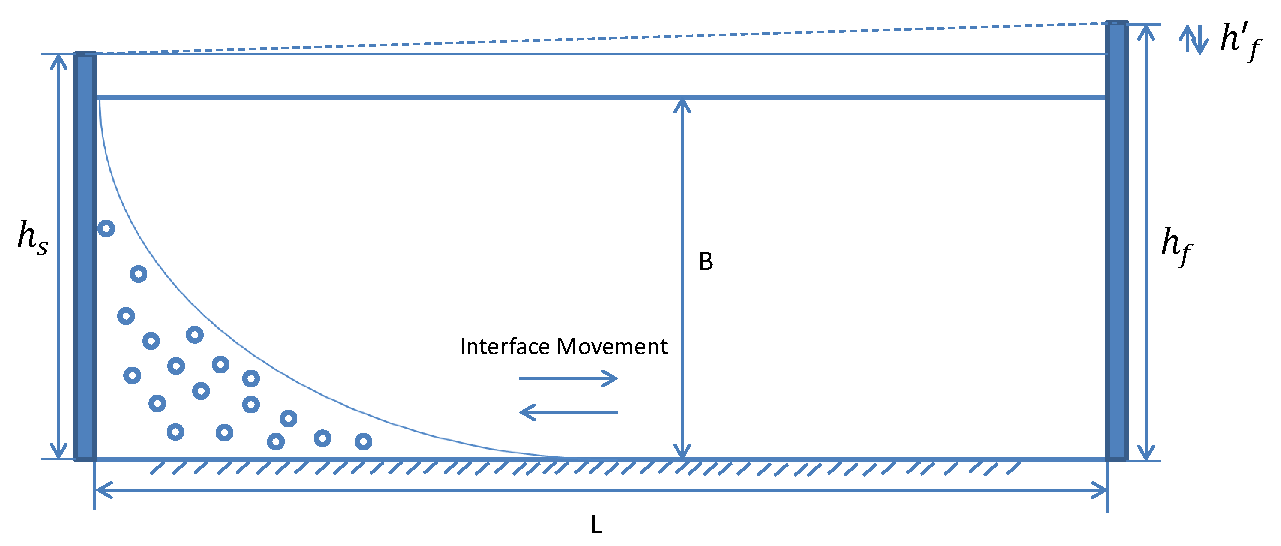
\includegraphics[width=1.0\textwidth]{figures/seawater_intrusion}
\caption{Conceptual model of the seawater intrusion and retreat}
\label{fig:seawater_intrusion}
\end{figure}

\subsection{Theoretical method}

\section{Result and discussion}

There are various bibliography styles available. You can select the style of your choice in the preamble of this document. These styles are Elsevier styles based on standard styles like Harvard and Vancouver. Please use Bib\TeX\ to generate your bibliography and include DOIs whenever available.

Here are two sample references: \cite{Feynman1963118,Dirac1953888}.

\section*{References}

\bibliography{mybibfile}

\end{document}